\documentclass[11  pt]{article} 
\usepackage[lmargin=1in,rmargin=1.75in,bmargin=1in,tmargin=1in]{geometry}  


% For hyperlinking everything
\usepackage{hyperref}
\hypersetup{
	colorlinks=true, %set true if you want colored links
	linktoc=all,     %set to all if you want both sections and subsections linked
	linkcolor=blue,  %choose some color if you want links to stand out
}


\usepackage[latin1]{inputenc}
\usepackage{amsmath}
\usepackage{mathrsfs}  
\usepackage{amsfonts}
\usepackage{amssymb}
\usepackage{graphicx}
\usepackage{subfig}
\usepackage{caption}
\usepackage{algorithm}
%\usepackage{algcompatible}
%\usepackage{algorithmicx}
\usepackage{algpseudocode}

\usepackage{titlesec}
\titleformat{\section}{\fontfamily{lmss}\fontsize{14}{15}\bfseries}{\thesection}{1em}{}
\titleformat{\subsection}{\fontfamily{lmss}\fontsize{12}{15}\bfseries}{\thesubsection}{1em}{}




\usepackage{amsthm}

\newtheoremstyle{noit}
{10pt}% <Space above>
{10pt}% <Space below>
{}% <Body font>
{}% <Indent amount>
{\bfseries}% <Theorem head font>
{.}% <Punctuation after theorem head>
{.5em}% <Space after theorem headi>
{}% <Theorem head spec (can be left empty, meaning `normal')>

\newtheoremstyle{example}
{10pt}% <Space above>
{10pt}% <Space below>
{}% <Body font>
{20pt}% <Indent amount>
{\bfseries}% <Theorem head font>
{.}% <Punctuation after theorem head>
{.5em}% <Space after theorem headi>
{}% <Theorem head spec (can be left empty, meaning `normal')>


\newtheoremstyle{indented}{20pt}{20pt}{\addtolength{\leftskip}{2.5em}}{}{\bfseries}{.}{.5em}{}


\newtheorem{theorem}{Theorem}
\numberwithin{theorem}{section}
\newtheorem{lemma}[theorem]{Lemma}
\newtheorem{corollary}[theorem]{Corollary}
\newtheorem{observation}{Observation}
%\numberwithin{observation}{section}
%\numberwithin{definition}{section}
\newtheorem{conjecture}{Conjecture}
\newtheorem{Qu}{Question}
\newcommand{\QU}{\begin{Qu}\normalfont}

\theoremstyle{noit}
\newtheorem{fact}{Fact}
\newtheorem{definition}{Definition}

\theoremstyle{indented}
\newtheorem{example}{Example}

\theoremstyle{indented}
\newtheorem{problem}{Problem}


%\newenvironment{proof}{\noindent{\bf Proof:} \hspace*{1em}}{
%    \hspace*{\fill} $\Box$ }
%\newenvironment{proof_of}[1]{\noindent {\bf Proof of #1:}
%    \hspace*{1em} }{\hspace*{\fill} $\Box$ }
%\newenvironment{proof_claim}{\begin{quotation} \noindent}{
%    \hspace*{\fill} $\diamond$ \end{quotation}}
\newcommand{\vs}[1]{\vspace{#1}}

\newcommand{\lecture}[2]{
 \noindent
\begin{center}
	\framebox{
		\vbox{
			\hbox to 5.78in { {\bf CSCE 411: Design and Analysis of Algorithms} \hfill  }
			\vspace{2mm}
			\hbox to 5.78in { {\Large \hfill Lecture #1\hfill} }
			\vspace{2mm}
			\hbox to 5.78in { {\it Date: #2 \hfill Lecturer: Nate Veldt} }
		}
	}
\end{center}
\vspace*{4mm}
}


\newcommand{\hw}[2]{
	\noindent
	\begin{center}
		\framebox{
			\vbox{
				\hbox to 5.78in { {\bf CSCE 411: Design and Analysis of Algorithms} \hfill  }
				\vspace{2mm}
				\hbox to 5.78in { {\Large \hfill Homework #1\hfill} }
				\vspace{2mm}
				\hbox to 5.78in { {\it Due date: #2 \hfil} }
			}
		}
	\end{center}
	\vspace*{4mm}
}



\newcommand{\under}[1]{\underline{\hspace{#1}}}
\setlength{\parindent}{0em}

%\usepackage[tagged]{accessibility}

% Graph terms
\newcommand{\vol}{\textbf{vol}}
\newcommand{\cut}{\textbf{cut}}


% Matrices
\newcommand{\mA}{\textbf{A}}
\newcommand{\mB}{\textbf{B}}

% vectors
\newcommand{\ve}{\textbf{e}}
\newcommand{\vx}{\textbf{x}}


% Other
\newcommand{\calN}{\mathcal{N}}

\usepackage{mathtools}
\DeclarePairedDelimiter\ceil{\lceil}{\rceil}
\DeclarePairedDelimiter\floor{\lfloor}{\rfloor}


\newcommand*{\aitem}{ \item[{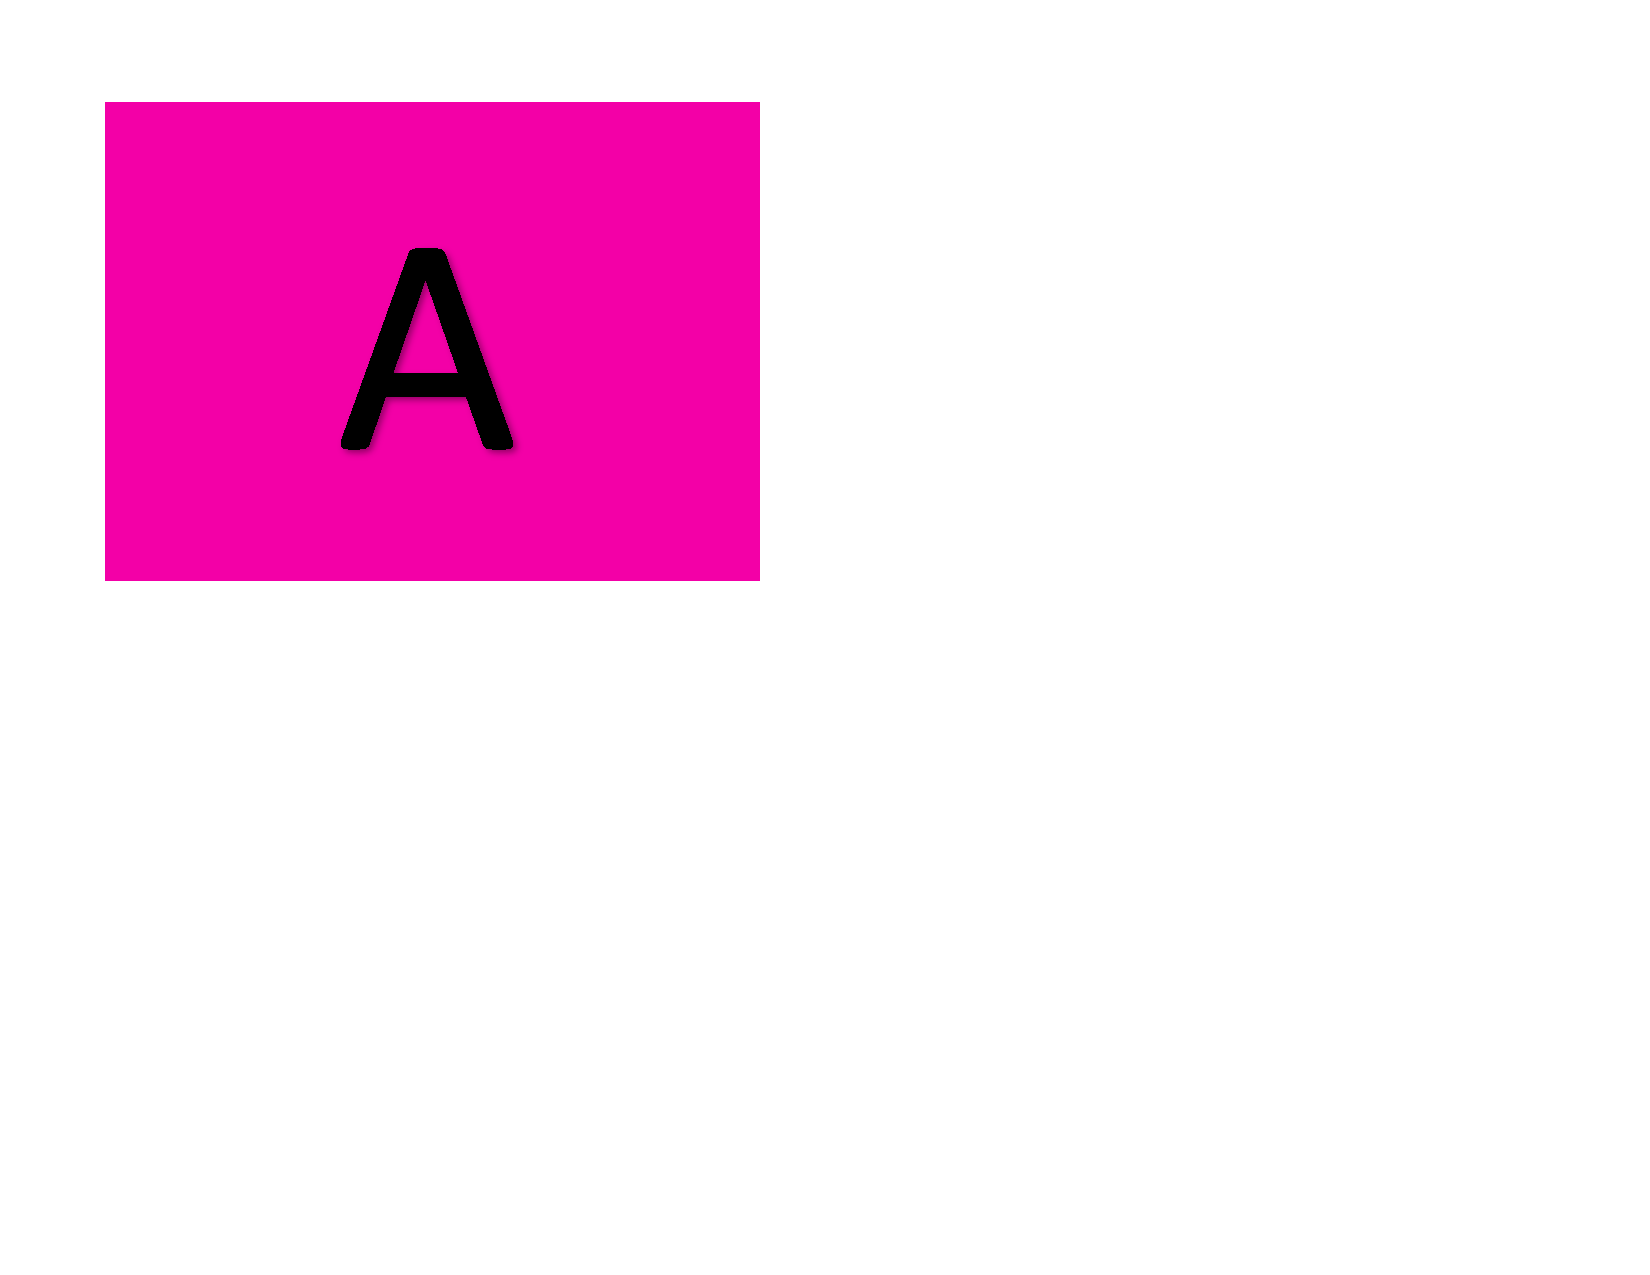
\includegraphics[width=0.8cm,height=0.5cm]{../../Lectures/figures/A}} ]  }
\newcommand*{\bitem}{ \item[{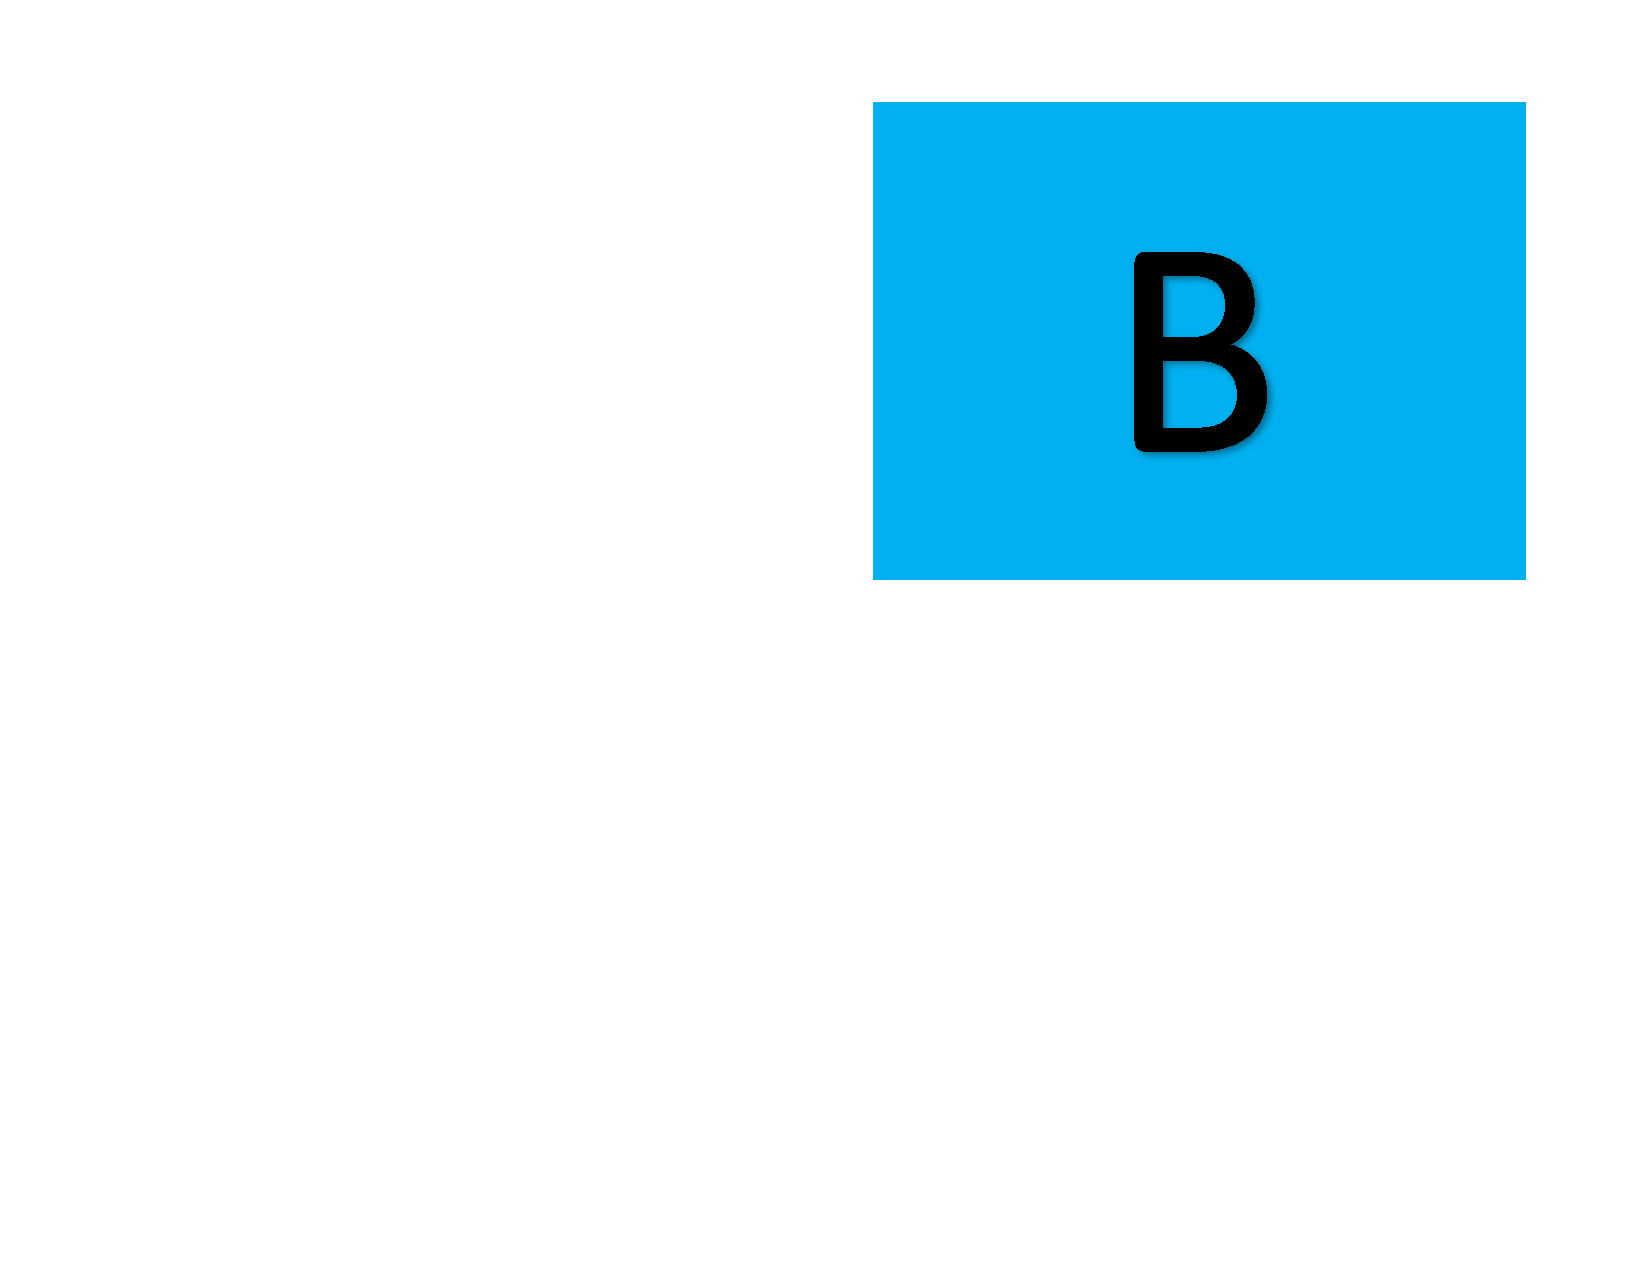
\includegraphics[width=0.8cm,height=0.5cm]{../../Lectures/figures/B}} ]  }
\newcommand*{\citem}{ \item[{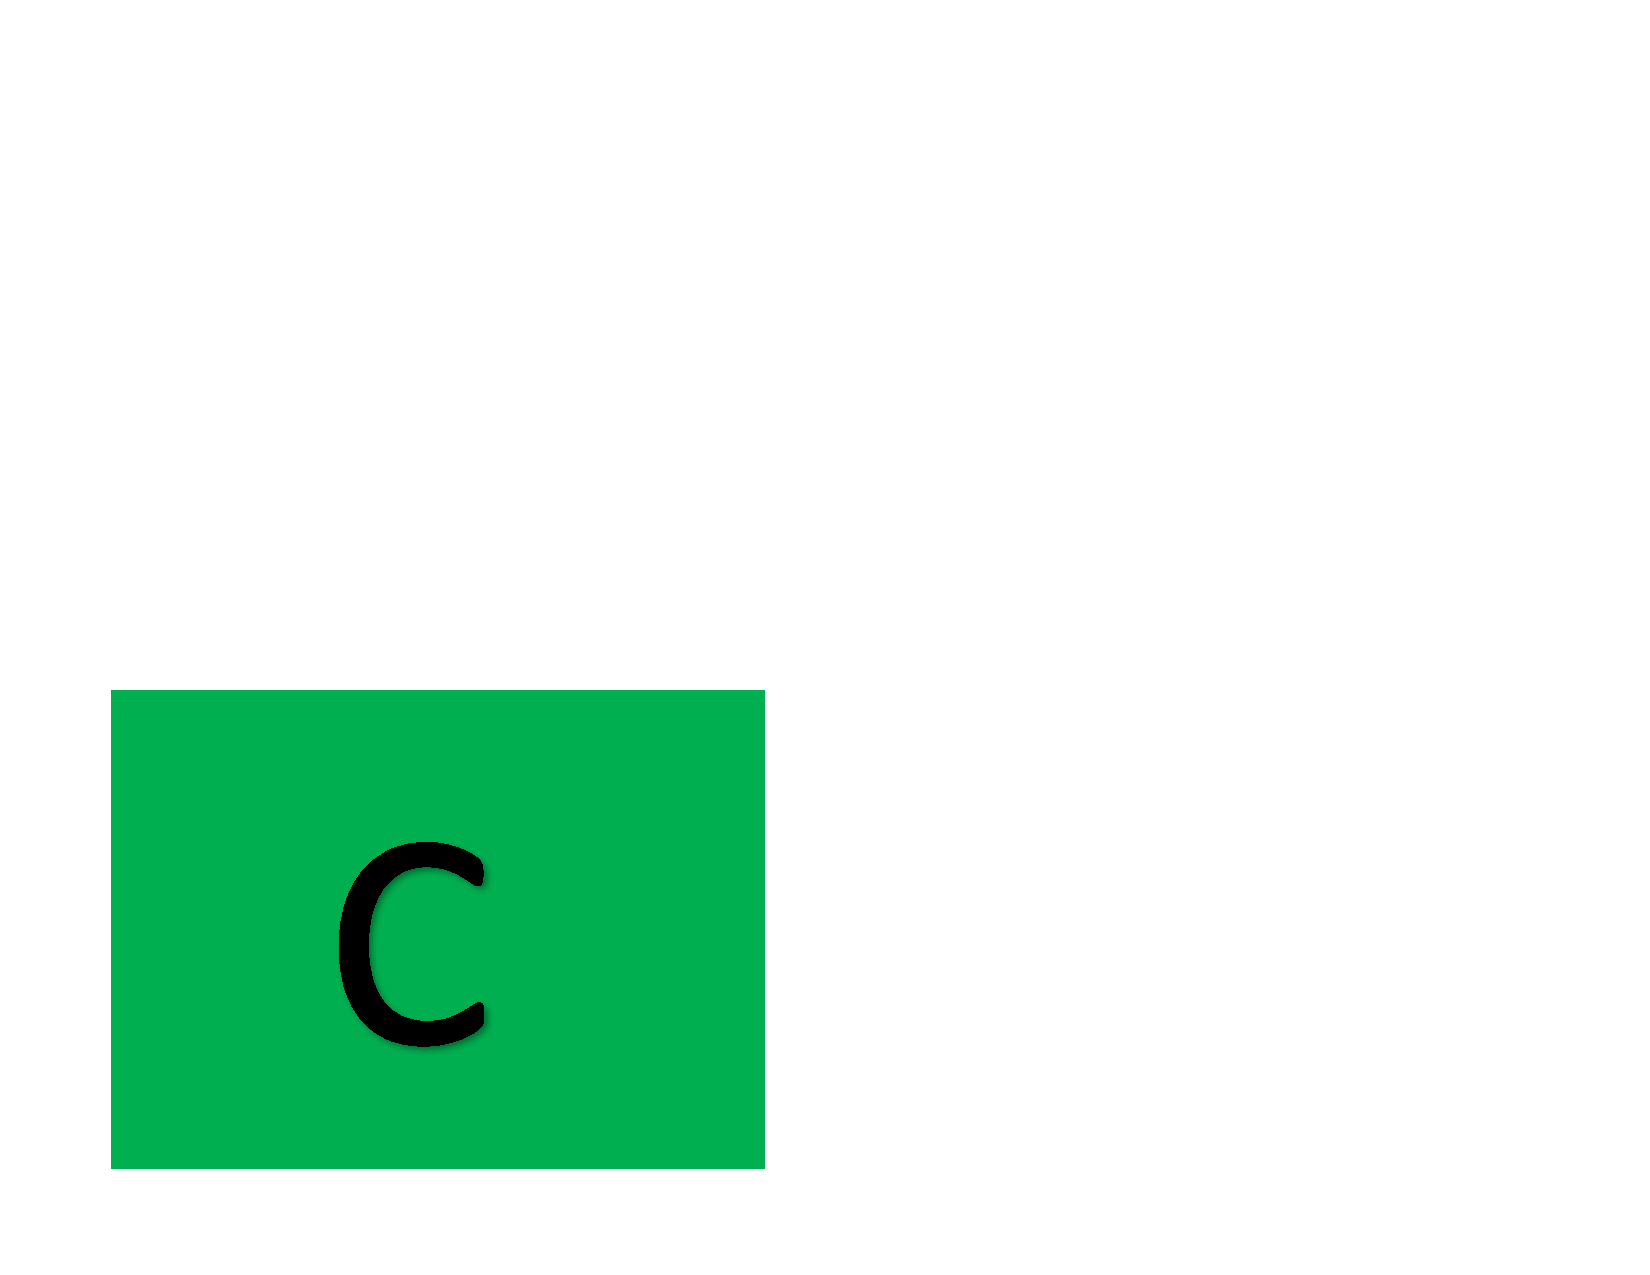
\includegraphics[width=0.8cm,height=0.5cm]{../../Lectures/figures/C}} ]  }
\newcommand*{\ditem}{ \item[{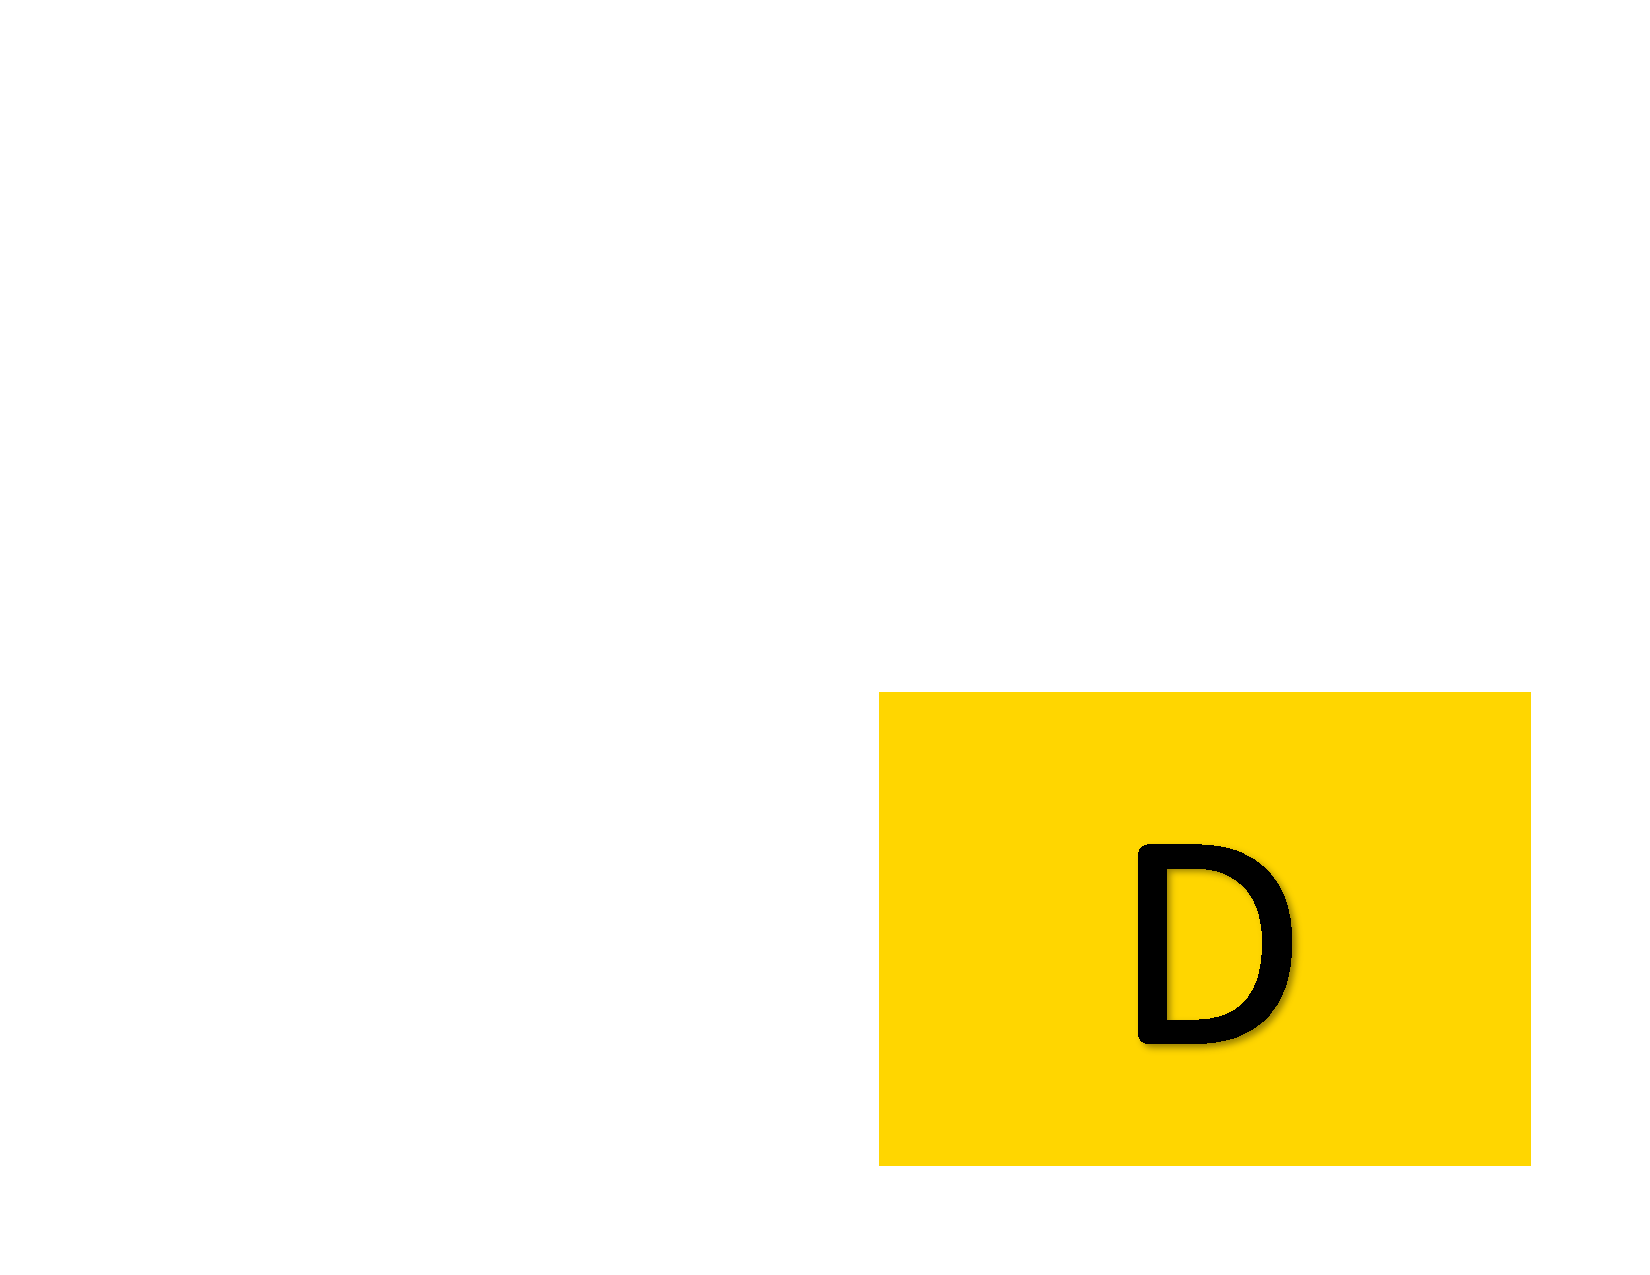
\includegraphics[width=0.8cm,height=0.5cm]{../../Lectures/figures/D}} ]  }
\newcommand*{\eitem}{ \item[{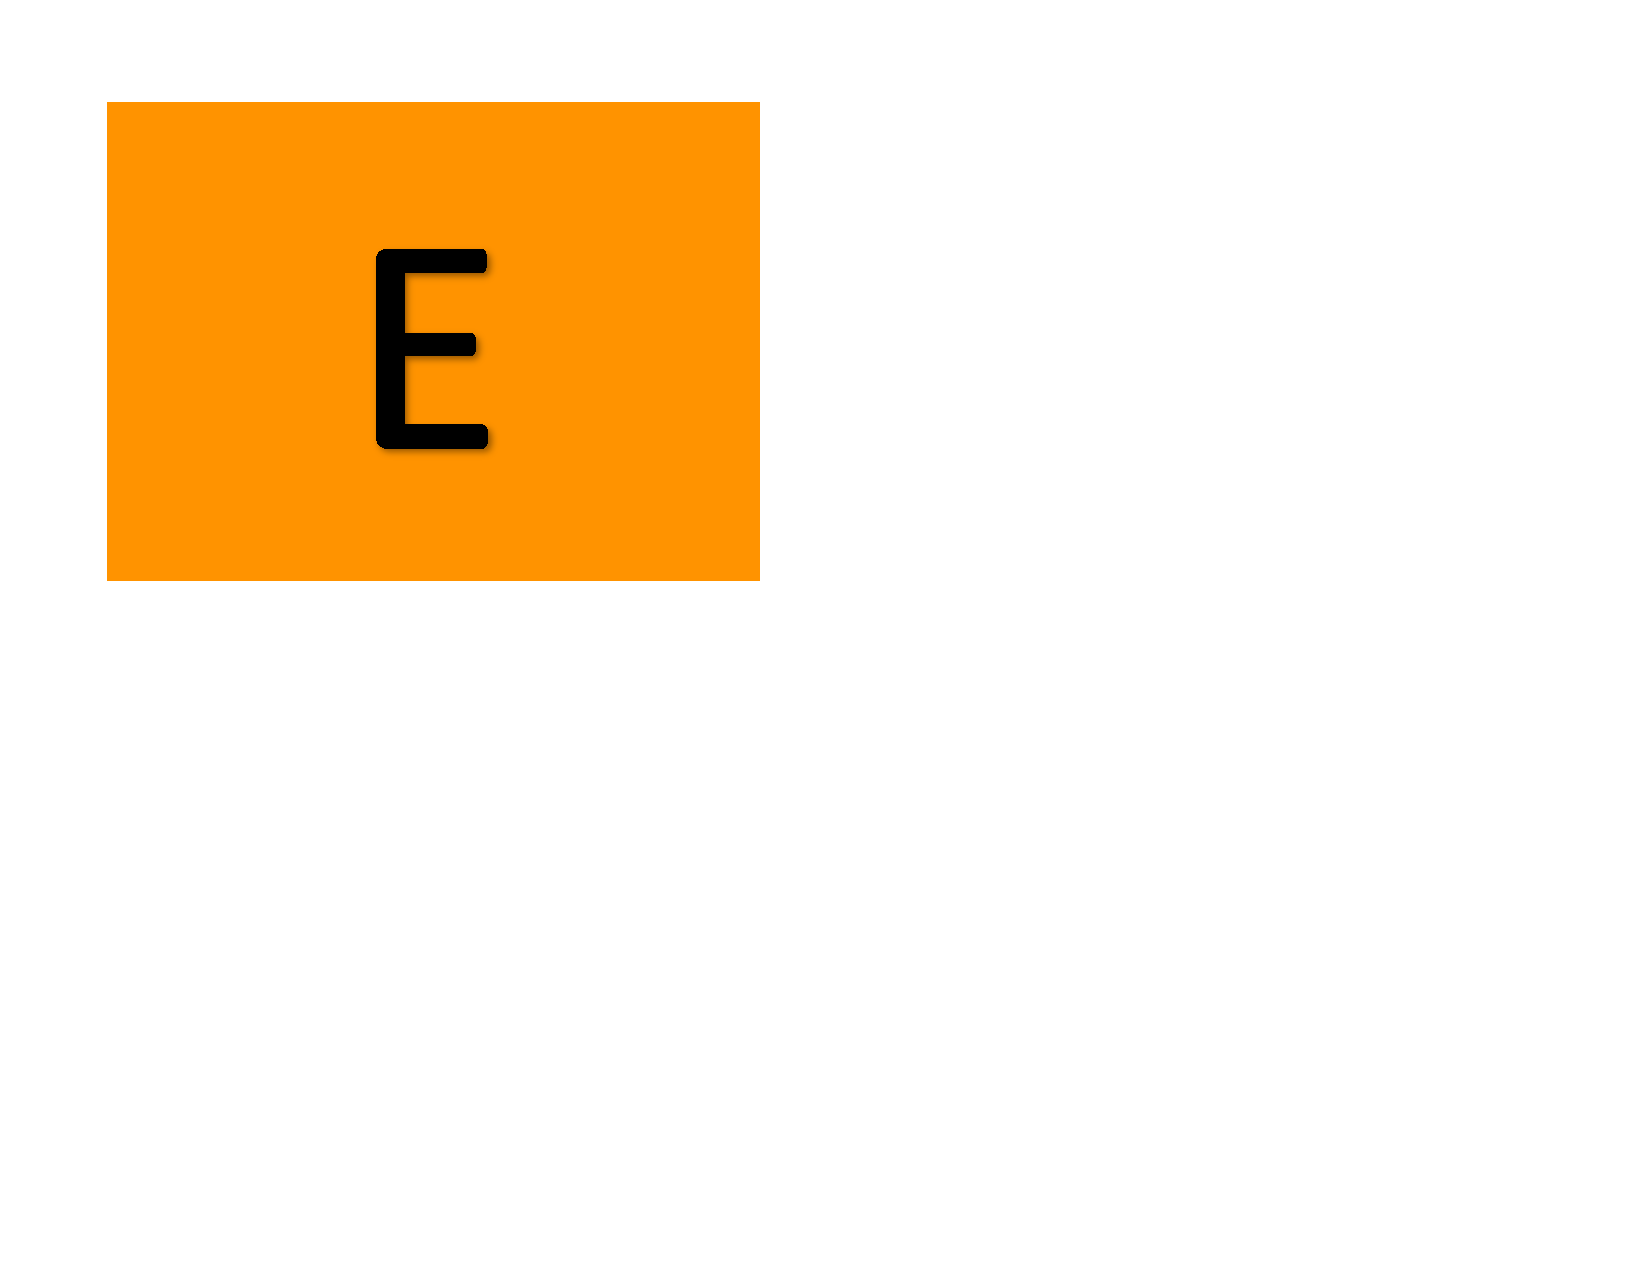
\includegraphics[width=0.8cm,height=0.5cm]{../../Lectures/figures/E}} ]  }
\newcommand*{\fitem}{ \item[{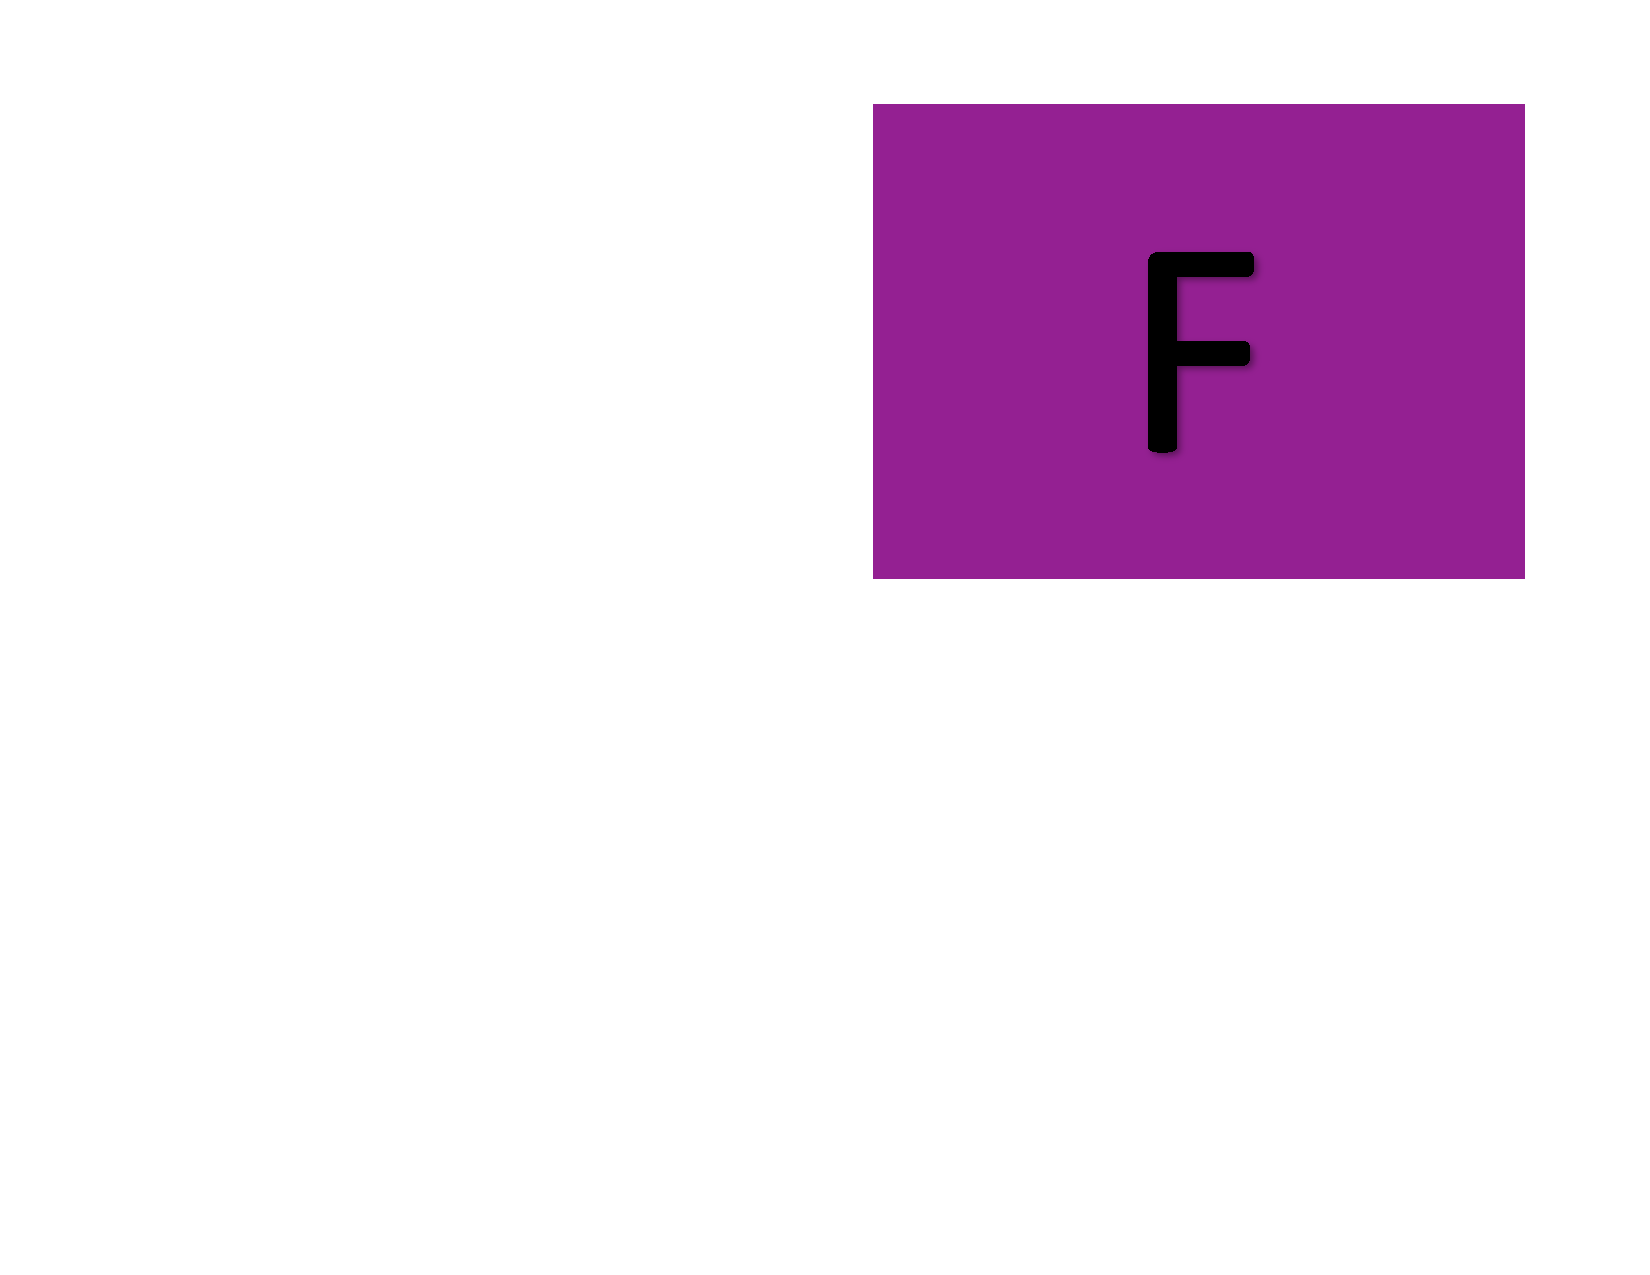
\includegraphics[width=0.8cm,height=0.5cm]{../../Lectures/figures/F}} ]  }


\newcommand{\hide}[1]{\underline{\phantom{#1 #1}}}

\usepackage{setspace}

\onehalfspacing

\begin{document}
	
	
	\lecture{7: Amortized Analysis}{February 4, 2025}
	
	\paragraph{Course Logistics}
	
	\begin{itemize}
		\item Amortized analysis: Chapter 17
		\item First test is next Thursday; Review will be held next Tuesday
	\end{itemize}
	
	\section{Simple Iterative Runtime Analysis}
	For simple iterative algorithms, a basic approach is to proving a runtime is to:
	%	multiply the number of iterations by the worst-case runtime for the inner loop.\\
	
	
	\newpage
	
	\section{The Multi-pop Stack}
	Consider a stack $S$ that has the following three operations
	\begin{itemize}
		\item $\textsc{Push}(S,v)$: puts value $v$ on the top of the stack
		\item $\textsc{Pop}(S)$: removes value on the top of the stack
		\item $\textsc{IsEmpty}(S)$: returns whether $S$ is empty
		\item $\textsc{Multipop}(S,k)$: 
		\begin{itemize}
			
			\item Calls \textsc{Pop} \\%$k$ times if stack has more than $k$ elements. 
			\item Pops \\%out all elements if $|S| < k$ 
			\item $k$ can be any integer number, different calls may involve different values of $k$
		\end{itemize}
	\end{itemize}
	
	\vfill
	
	\QU
	Assume that a single push or pop operation takes $O(1)$ time. If we start with an empty stack, what is the worst-case runtime bound we obtain for applying $n$ pop, push, and multipop operations, by applying a simple iterative runtime analysis?
	\begin{itemize}
		\aitem $O(1)$
		\bitem $O(n)$ 
		\citem $O(nk)$
		\ditem $O(n^2)$
	\end{itemize}
\end{Qu}

\pagebreak

\section{Amortized Analysis}
In \emph{amortized analysis}, we obtain improved runtime bounds for iterative methods by bounding the \hide{average cost of each iteration.}

\subsection{Technique 1: Aggregate Analysis}
\begin{algorithm}[t]
	\textsc{PushPopFun}($n$)
	\begin{algorithmic}
		\State Initialize empty multipop stack $S$
		\For{$i = 1$ to $n$}
		\State Generate random number $b \in [0,1]$
		\If{$b < 1/3$}
		\State $\textsc{Push}(S,1)$
		\ElsIf{$b \in [1/3, 2/3)$}
		\State $\textsc{Pop}(S)$
		\Else
		\State Generate random integer $k \in [1,n]$
		\State $\textsc{MultiPop}(S,k)$
		\EndIf
		\EndFor
	\end{algorithmic}
\end{algorithm}

Let $T(n)$ be:

\begin{center}
	\hide{the total number of individual push/pop }% operations called during \textsc{PushPopFun}($n$). \\
\end{center} 

Note that $\textsc{MultiPop}(S,k)$ performs \hide{$\min{k, |S|}$ such} \\

The average cost per iteration (or \emph{amortized cost}) is then\\  %$T(n)/n$. \\

\begin{theorem}
	\textsc{PushPopFun}($n$) makes at most \hide{$O(n)$} individual push/pop operations. 
\end{theorem}

\pagebreak

\paragraph{An important distinction}
Our runtime analysis did not involve probabilistic reasoning. There are other notions of ``average cost'' for probabilistic algorithms, but we are not considering these. Our analysis holds independent of the random numbers generated in Algorithm \textsc{PushPopFun}.

\newpage

\subsection{Another approach for analyzing multipop stacks}
If $S$ is a multipop stack, and if it starts empty, then it is possible to pop an element $v$ only if \emph{we previously we pushed $v$ onto $S$.}\\

\emph{Key idea:} Let's ``pay'' in advance for an eventual \textsc{Pop} of that element.
\begin{itemize}
	\item Whenever we push a new element,\hide{ just pretend this }\\ %costs 2 operations
	\item If/when that element is popped \hide{we have already paid} \\
	\item This is true whether we called \hide{\textsc{Pop} or \textsc{Multipop}}\\
	
	%	If we pretend \textsc{Push} ``costs'' 2, and \textsc{Pop} or \textsc{Multipop} are ``free'', it all works out.
	
	\item In $n$ iterations, there are at most $n$ push operations and so \hide{ the cost is a}
\end{itemize}

\emph{Alternative view:} Each time we ``overpay'' for a push, we put money in the bank to pay for future pops.



\newpage
\subsection{Technique 2: The accounting method}
Define:
\begin{itemize}
	\item $c_i = $ the actual cost incurred at step $i$ 
	\item $\hat{c}_i$ the \hide{\emph{amortized cost we assign }}
\end{itemize}
Here's how the accounting method works:
\begin{itemize}
	\item The runtime we want to bound is:\\ %$\sum_{i = 1}^n c_i$
	\item We choose convenient $\hat{c}_i$ for each iteration so that
	\vs{3cm}
\end{itemize}

%\textbf{An intuitive interpretation} We use some amortized costs to ``pay in advance'' for other future operations.\\

\paragraph{Multipop Stack Example}
In this example, 
$$c_i = \text{number of pop/push operations in iteration $i$}.$$

\begin{equation*}
	\hat{c}_i = \begin{cases}
		\hide{num} & \text{if we push in step $i$} \\ \\
		\hide{num} & \text{if we pop or multipop in step $i$}
	\end{cases}
\end{equation*}

\pagebreak


\subsection{Technique 3: The potential method}
In the potential method, we identify some data structure and define:
\begin{itemize}
	\item $c_i$: the actual cost incurred at step $i$ 
	\item $D_i$: the state of a  data structure after the $i$th iteration
	\item $\Phi$: potential function defined on data structure; $\Phi(D_i)$ is a real number
	\item $\hat{c}_i = \hide{c_i + \Phi(D_i) - \Phi(D_{i-1})}$ is the amortized cost
\end{itemize}
If \hide{$\Phi(D_n) \geq \Phi(D_0)$}, we can bound actual cost in terms of amortized costs as follows:


\vfill

%Bounding $\sum \hat{c}_i$ should be easier, and this will bound the total cost.

\pagebreak
\paragraph{Multipop Stack Example} 
Define:


$c_i$ = number of push/pop operations at step $i$

The data structure is \hide{the stack}  \\% the stack, which has state $D_i$ after step $i$ \\

Define $\Phi(D_i) = \hide{|S|}$ \\

Notice then that 
$$\Phi(D_i) - \Phi(D_0) =  \hide{\Phi(D_n) - 0 = } $$

At step $i$, we ``pay'' $\hat{c}_i = c_i + \Phi(D_i) - \Phi(D_{i-1})$\\


\emph{In-Class Activity}
\begin{enumerate}
	\item Write down the amortized cost $\hat{c}_i$ in three different cases: 
	\begin{enumerate}
		\item In iteration $i$, a pop happens
		\item In iteration $i$, a push happens
		\item In iteration $i$, a multipop happens
	\end{enumerate}
	\item Bound the runtime using step 1.
\end{enumerate}



\pagebreak
\paragraph{Similarities and differences with the accounting method}
\begin{itemize}
	\item Similarity: both store ``credit'' and ``pay'' ahead of time
	\item The accounting method stores credit in individual steps %(e.g., each push operation adds credit).
	\item The potential method stores credit as ``potential'' in a data structure
	\item For potential method, choose $D_i$ and $\Phi$ and prove $\Phi(D_i) \geq \Phi(D_0)$. \hide{$\hat{c}_i$ is given}\\
	\item For accounting, there is no $D_i$ or $\Phi$. You must choose $\hat{c}_i$ and prove \hide{$\sum \hat{c}_i \geq \sum c_i$}
	\item For both, bound \hide{$\sum_{i = 1}^n \hat{c}_i$} to prove runtime guarantee.
\end{itemize}

\pagebreak

\section{Representing numbers in binary}
We represent a number $x \in \mathbb{N}$ in binary by a vector of bits $A[0..k]$, where $A[i] \in \{0,1\}$ and
\begin{equation*}
	x = \sum_{i = 0}^k  A[i] \cdot 2^i
\end{equation*}

%	\paragraph{Examples}


\pagebreak 

\section{The Binary Counter Problem}
Let \textsc{Increment} be an algorithm that takes in a binary vector and adds one to the binary number that it represents.
\begin{algorithm}
	\textsc{Increment}($A$)
	\begin{algorithmic}
		\State $i = 0$
		\While{$i < A.length$ and $A[i] == 1$}
		\State $A[i] = 0$
		\State $i = i+1$
		\EndWhile
		\If{$i < A.length$}
		\State
		\State \hide{$A[i] = 1$}
		\State
		\EndIf
	\end{algorithmic}
\end{algorithm}

\vfill

\QU
If $A$ is length $k$ binary vector, what is the worst-case runtime for calling $\textsc{Increment}(A)$?
\begin{itemize}
	\aitem $O(1)$
	\bitem $O(\log k)$
	\citem $O(k)$
	\ditem $O(n)$
\end{itemize}
\end{Qu}

\pagebreak
\subsection{The actual cost of each iteration}
Assume it takes $O(1)$ time to check an entry of $A$ or to flip its bit. At each step, the runtime is then just $O(\text{number of flipped bits})$, so we will say the cost of an iteration is 
\begin{center}
$c_i$ = \hide{number of flipped bits in iteration $i$.}
\end{center}

\emph{Key idea:} Separate the costs that happen \hide{at each entry $A[j]$}\\ \\

\vs{1cm} 

{\Huge
\begin{tabular}{ l || p{1cm} | p{1cm} | p{1cm} | p{1cm} | p{1cm} |}
	\hline
	0& 	0 & 0 & 0 & 0 & 0\\
	\hline 
	1& 	0 & 0 & 0 & 0 & 1\\
	\hline 
	2& 	0 & 0 & 0 & 1 & 0\\
	\hline 
	3& 	0 & 0 & 0 & 1 & 1\\
	\hline 
	4& 	0 & 0 & 1 & 0 & 0\\
	\hline 
	5& 	0 & 0 & 1 & 0 & 1\\
	\hline 
	6& 	0 & 0 & 1 & 1 & 0\\
	\hline 
	7& 	0 & 0 & 1 & 1 & 1\\
	\hline 
	8& 	0 & 1 & 0 & 0 & 0\\
	\hline 
	9& 	0 & 1 & 0 & 0 & 1\\
	\hline 
	10& 	0 & 1 & 0 & 1 & 0\\
	\hline 
	11& 	0 & 1 & 0 & 1 & 1\\
	\hline 
\end{tabular}
}

\newpage 

\subsection{Technique 1: Aggregate Analysis}
Let $T(n)$ be the total number of number of flipped bits in $n$ increments.

\QU
Look at the table on the last page, and observe how often the bit in position $A[j]$ is flipping. If you wish, fill in the number of total flipped bits at each increment. What is the total cost of calling \textsc{Increment} $n$ times?
\begin{itemize}
\aitem $O(n)$
\bitem $O(k)$
\citem $O(nk)$ 
\ditem $O(n^2)$
\end{itemize}
\end{Qu}


\pagebreak
\subsection{Technique 2: The accounting method}
\begin{itemize}
\item $c_i = $ the actual number of bits flipped
\item $\hat{c}_i$ amortized cost for flipping bits: \hide{\$2 for setting 0 to 1}
\end{itemize}
{\Huge
\begin{tabular}{ l || p{1cm} | p{1cm} | p{1cm} | p{1cm} | p{1cm} |}
\hline
0& 	0 & 0 & 0 & 0 & 0\\
\hline 
1& 	0 & 0 & 0 & 0 & 1\\
\hline 
2& 	0 & 0 & 0 & 1 & 0\\
\hline 
3& 	0 & 0 & 0 & 1 & 1\\
\hline 
4& 	0 & 0 & 1 & 0 & 0\\
\hline 
5& 	0 & 0 & 1 & 0 & 1\\
\hline 
6& 	0 & 0 & 1 & 1 & 0\\
\hline 
7& 	0 & 0 & 1 & 1 & 1\\
\hline 
8& 	0 & 1 & 0 & 0 & 0\\
\hline 
9& 	0 & 1 & 0 & 0 & 1\\
\hline 
\end{tabular}
}
\begin{algorithm}
\textsc{Increment}($A$)
\begin{algorithmic}
\State $i = 0$
\While{$i < A.length$ and $A[i] == 1$}
\State $A[i] = 0$
\State $i = i+1$
\EndWhile
\If{$i < A.length$}
\State $A[i] = 1$
\EndIf
\end{algorithmic}
\end{algorithm}

\pagebreak
\subsection{Technique 3: The potential method}

\textbf{Step 0:} Identify data structure, potential function, and costs.
\begin{itemize}
\item $c_i$: the actual number of flipped bits at iteration $i$
\item data structure: \hide{the counter $A$}, with state $D_i$ after iteration $i$
\item $\Phi(D_i) = b_i$ = \hide{number of 1's in the counter} % after iteration $i$
\item $\hat{c}_i = $ \hide{is the amortized cost}
\end{itemize}

\textbf{Step 1: Check that $\Phi(D_i) \geq \Phi(D_0)$}

\vspace{3cm}

\textbf{Step 2: Compute and bound amortized costs}\\

Let $t_i$ be the number of bits that are set to $0$ (\emph{while} loop in algorithm) in iteration $i$.\\

If $b_i = 0$, this means we had $A = [1 \; 1 \; 1 \; \cdots \; 1]$ in iteration $i$, and incrementing turned it into $A = [0 \; 0 \; 0 \; \cdots \; 0]$, meaning $b_{i-1} = t_i = k$. \\

\begin{Qu}
If $b_i > 0$, which of these is the right expression for $b_i$?
\begin{itemize}
\aitem $b_i = b_{i-1} + 1$
\bitem $b_i = t_i + 1$
\citem $b_i = b_{i-1} + t_i$ 
\ditem $b_i = b_{i-1} - t_i$ 
\eitem $b_i = b_{i-1} + t_i + 1$
\fitem $b_i = b_{i-1} - t_i + 1$
\end{itemize}
\end{Qu}

\pagebreak
Whether or not $b_i = 0$, we have a bound of \hide{$b_i \leq b_{i-1} - t_i  + 1$.}\\

We can then compute the amortized cost and overall runtime bound:


%\pagebreak
%\subsection{Binary counter problem: potential method}
%
%\textbf{Step 0:} Identify data structure, potential function, and costs.
%\begin{itemize}
%	\item $c_i$: the actual number of flipped bits at iteration $i$
%	\item data structure: the counter $A$, with state $D_i$ after iteration $i$
%	\item $\Phi(D_i) = b_i$ = number of 1's in the counter after iteration $i$
%	\item $\hat{c}_i = c_i + \Phi(D_i) - \Phi(D_{i-1})$ is the amortized cost
%\end{itemize}
%
%\textbf{Step 1: Check that $\Phi(D_i) \geq \Phi(D_0)$}
%
%At step zero we know $\Phi(D_0) = 0$, since there are no 1's in the binary representation of 0. \\
%
%At step $i$, we still have $\Phi(D_i) \geq 0$, since we can't have a negative number of zeros. \\
%
%
%\textbf{Step 2: Compute and bound amortized costs}\\
%
%Let $t_i$ be the number of bits that are set to $0$ (\emph{while} loop in algorithm) in iteration $i$.\\
%
%If $b_i = 0$, this means we had $A = [1 \; 1 \; 1 \; \cdots \; 1]$ in iteration $i$, and incrementing turned it into $A = [0 \; 0 \; 0 \; \cdots \; 0]$, meaning $b_{i-1} = t_i = k$. \\
%
%\begin{Qu}
%	If $b_i > 0$, which of these is the right expression for $b_i$?
%	\begin{itemize}
%		\aitem $b_i = b_{i-1} + 1$
%		\bitem $b_i = b_{i-1} + t_i + 1$
%		\citem $b_i = b_{i-1} - t_i + 1$
%		\ditem $b_i = b_{i-1} + t_i$ 
%		\eitem $b_i = b_{i-1} - t_i$ 
%		\fitem $b_i = t_i + 1$
%	\end{itemize}
%\end{Qu}
%
%\pagebreak
%Whether or not $b_i = 0$, we have a bound of \hide{$b_i \leq b_{i-1} - t_i  + 1$.}\\
%
%We can then compute the amortized cost and overall runtime bound:
%
%
%
%\pagebreak
%\textbf{What happens if we do not start with an empty counter?} 
%
%\vs{1cm}
%
%This means that \hide{$\Phi(D_0) = b_0 \geq 1$.}
%



\end{document}
